\section{CTKInterpreter\-Startup  Class Reference}
\label{classCTKInterpreterStartup}\index{CTKInterpreterStartup@{CTKInterpreter\-Startup}}
{\tt \#include $<$CTKInterpreter\-Startup.h$>$}

Inheritance diagram for CTKInterpreter\-Startup::\begin{figure}[H]
\begin{center}
\leavevmode
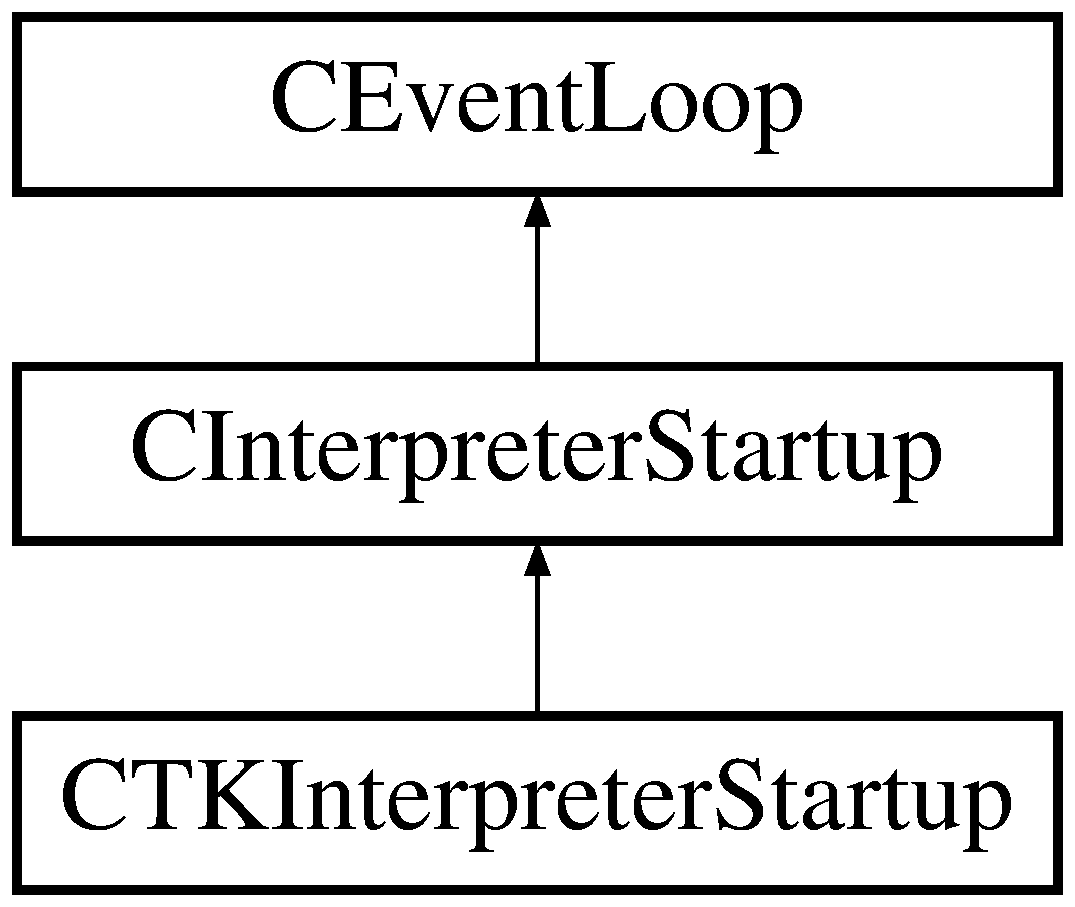
\includegraphics[height=3cm]{classCTKInterpreterStartup}
\end{center}
\end{figure}
\subsection*{Public Methods}
\begin{CompactItemize}
\item 
{\bf CTKInterpreter\-Startup} ()
\item 
virtual {\bf $\sim$CTKInterpreter\-Startup} ()
\end{CompactItemize}
\subsection*{Static Protected Methods}
\begin{CompactItemize}
\item 
int {\bf Tk\_\-Init} (Tcl\_\-Interp $\ast$p\-Interp)
\end{CompactItemize}
\subsection*{Private Methods}
\begin{CompactItemize}
\item 
{\bf CTKInterpreter\-Startup} (const CTKInterpreter\-Startup \&a\-CTKInterpreter\-Startup)
\begin{CompactList}\small\item\em Copy Constructor illegal, private, unimplemented.\item\end{CompactList}\item 
CTKInterpreter\-Startup \& {\bf operator=} (const CTKInterpreter\-Startup \&a\-CTKInterpreter\-Startup)
\begin{CompactList}\small\item\em Operator= Assignment Operator illegal, private, unimplemented.\item\end{CompactList}\item 
int {\bf operator==} (const CTKInterpreter\-Startup \&a\-CTKInterpreter\-Startup) const
\begin{CompactList}\small\item\em Operator== Equality Operator illegal, private, unimplemented.\item\end{CompactList}\item 
virtual int {\bf operator()} (int argc, char $\ast$$\ast$argv)
\end{CompactItemize}


\subsection{Detailed Description}
Encapsulates the startup of a Tk/wish interpreter. An application must subclass this, Implement Register\-Extensions. 



Definition at line 311 of file CTKInterpreter\-Startup.h.

\subsection{Constructor \& Destructor Documentation}
\index{CTKInterpreterStartup@{CTKInterpreter\-Startup}!CTKInterpreterStartup@{CTKInterpreterStartup}}
\index{CTKInterpreterStartup@{CTKInterpreterStartup}!CTKInterpreterStartup@{CTKInterpreter\-Startup}}
\subsubsection{\setlength{\rightskip}{0pt plus 5cm}CTKInterpreter\-Startup::CTKInterpreter\-Startup ()\hspace{0.3cm}{\tt  [inline]}}\label{classCTKInterpreterStartup_a0}




Definition at line 314 of file CTKInterpreter\-Startup.h.\index{CTKInterpreterStartup@{CTKInterpreter\-Startup}!~CTKInterpreterStartup@{$\sim$CTKInterpreterStartup}}
\index{~CTKInterpreterStartup@{$\sim$CTKInterpreterStartup}!CTKInterpreterStartup@{CTKInterpreter\-Startup}}
\subsubsection{\setlength{\rightskip}{0pt plus 5cm}virtual CTKInterpreter\-Startup::$\sim$CTKInterpreter\-Startup ()\hspace{0.3cm}{\tt  [inline, virtual]}}\label{classCTKInterpreterStartup_a1}




Definition at line 315 of file CTKInterpreter\-Startup.h.\index{CTKInterpreterStartup@{CTKInterpreter\-Startup}!CTKInterpreterStartup@{CTKInterpreterStartup}}
\index{CTKInterpreterStartup@{CTKInterpreterStartup}!CTKInterpreterStartup@{CTKInterpreter\-Startup}}
\subsubsection{\setlength{\rightskip}{0pt plus 5cm}CTKInterpreter\-Startup::CTKInterpreter\-Startup (const CTKInterpreter\-Startup \& {\em a\-CTKInterpreter\-Startup})\hspace{0.3cm}{\tt  [private]}}\label{classCTKInterpreterStartup_c0}


Copy Constructor illegal, private, unimplemented.



\subsection{Member Function Documentation}
\index{CTKInterpreterStartup@{CTKInterpreter\-Startup}!operator()@{operator()}}
\index{operator()@{operator()}!CTKInterpreterStartup@{CTKInterpreter\-Startup}}
\subsubsection{\setlength{\rightskip}{0pt plus 5cm}int CTKInterpreter\-Startup::operator() (int {\em argc}, char $\ast$$\ast$ {\em argv})\hspace{0.3cm}{\tt  [private, virtual]}}\label{classCTKInterpreterStartup_c3}


Starts up the Tk interpreter.

\begin{CompactItemize}
\item 
Calls On\-Initialize to allow users to do early initialization.\item 
Starts the Tk interpreter by callling Tk\_\-Main.\end{CompactItemize}
The static member Tk\_\-Init is passed as  the application initialization function.\begin{Desc}
\item[Parameters: ]\par
\begin{description}
\item[{\em 
argc}]The number of \char`\"{}command line\char`\"{} parameters \item[{\em 
argv}]Vector of pointers to the \char`\"{}command line\char`\"{} parameter strings. \end{description}
\end{Desc}


Implements {\bf CInterpreter\-Startup} {\rm (p.\,\pageref{classCInterpreterStartup_c0})}.

Definition at line 307 of file CTKInterpreter\-Startup.cpp.

References CInterpreter\-Startup::On\-Initialize(), and Tk\_\-Init().\index{CTKInterpreterStartup@{CTKInterpreter\-Startup}!operator=@{operator=}}
\index{operator=@{operator=}!CTKInterpreterStartup@{CTKInterpreter\-Startup}}
\subsubsection{\setlength{\rightskip}{0pt plus 5cm}CTKInterpreter\-Startup\& CTKInterpreter\-Startup::operator= (const CTKInterpreter\-Startup \& {\em a\-CTKInterpreter\-Startup})\hspace{0.3cm}{\tt  [private]}}\label{classCTKInterpreterStartup_c1}


Operator= Assignment Operator illegal, private, unimplemented.

\index{CTKInterpreterStartup@{CTKInterpreter\-Startup}!operator==@{operator==}}
\index{operator==@{operator==}!CTKInterpreterStartup@{CTKInterpreter\-Startup}}
\subsubsection{\setlength{\rightskip}{0pt plus 5cm}int CTKInterpreter\-Startup::operator== (const CTKInterpreter\-Startup \& {\em a\-CTKInterpreter\-Startup}) const\hspace{0.3cm}{\tt  [private]}}\label{classCTKInterpreterStartup_c2}


Operator== Equality Operator illegal, private, unimplemented.

\index{CTKInterpreterStartup@{CTKInterpreter\-Startup}!Tk_Init@{Tk\_\-Init}}
\index{Tk_Init@{Tk\_\-Init}!CTKInterpreterStartup@{CTKInterpreter\-Startup}}
\subsubsection{\setlength{\rightskip}{0pt plus 5cm}int CTKInterpreter\-Startup::Tk\_\-Init (Tcl\_\-Interp $\ast$ {\em p\-Interp})\hspace{0.3cm}{\tt  [static, protected]}}\label{classCTKInterpreterStartup_e0}


Called by Tk\_\-Main to do application  specific initialization.

\begin{CompactItemize}
\item 
Establishes object context by invoking {\bf CEvent\-Loop::get\-Instance}() {\rm (p.\,\pageref{classCEventLoop_d0})} \item 
Invokes Register\-Extensions so that applicaiton packages and commands can be registered on the interpreter.\item 
Finally returns to the Tk event loop..\end{CompactItemize}
\begin{Desc}
\item[Parameters: ]\par
\begin{description}
\item[{\em 
p\-Interp}]Pointer to the Tcl interpreter created by Tk\_\-Main. \end{description}
\end{Desc}


Definition at line 342 of file CTKInterpreter\-Startup.cpp.

References CEvent\-Loop::get\-Instance(), CInterpreter\-Startup::Register\-Extensions(), CInterpreter\-Startup::set\-Interpreter(), and Tk\_\-Init().

Referenced by operator()(), and Tk\_\-Init().

The documentation for this class was generated from the following files:\begin{CompactItemize}
\item 
{\bf CTKInterpreter\-Startup.h}\item 
{\bf CTKInterpreter\-Startup.cpp}\end{CompactItemize}
